\chapter{HCQT: widmo ułożone harmonicznie}\label{rozdz:hcqt}

\section{Pomysł: niech każdy kandydat widzi swoje alikwoty w jednym miejscu}

Mamy widmo $\abs{X[k]}$ okna dźwięku (rozdział~\ref{rozdz:fourier}) i wiemy, że nuta to szereg alikwotów (rozdział~\ref{rozdz:alikwoty}).
Chcemy, żeby sieć uczyła się ,,wzorca nuty''. Gdyby ułożyć widmo tak, by dla \emph{każdego kandydata na wysokość} wszystkie jego
alikwoty leżały w tym samym miejscu tensora, zwykła konwolucja (rozdział~\ref{rozdz:siec}) mogłaby je porównywać bez żadnej
kombinatoryki. Tak działa HCQT (ang.\ \emph{harmonic constant-Q transform}): to stos kopii widma, z których $h$-ta jest „ściśnięta” $h$-krotnie.
Nasz opis opiera się na pomyśle Bittnera i in.\ (2017).

Po tym rozdziale umiesz: (i)~zdefiniować wartość HCQT w binie $p$ kanału $h$, (ii)~policzyć decybele i normalizację,
(iii)~udowodnić, że cechy nie zależą od głośności nagrania, (iv)~udowodnić, że kanały to przesunięte kopie jednego widma, (v)~odczytać kształt $X\in\R^{T\times9\times159}$.

\section{Biny logarytmiczne i alikwoty}

Zamiast równych odstępów w hercach (jak w DFT) używamy równych odstępów w \emph{półtonach}: wprost z rozdziału~\ref{rozdz:alikwoty} wiemy, że wtedy
wzorzec alikwotów jest niezmienniczy względem przesunięcia.

\haslo{bin logarytmiczny}
\begin{definicja}[Bin wysokości i jego częstotliwość]\label{def:bin}
Niech $b=3$ (liczba binów na półton) i $m_{\min}=36$. Bin o numerze $p=0,1,\dots,158$ ma wysokość
$m_p=m_{\min}+\dfrac{p-1}{3}$ (w skali MIDI) i częstotliwość środkową $f(p)=440\cdot2^{(m_p-69)/12}$. Bin $p=3s+1$ jest środkiem półtonu $s=0,\dots,52$ (nuta MIDI $36+s$);
biny $3s$ i $3s+2$ leżą $33{,}3$ centa niżej i wyżej.
\end{definicja}

\begin{przyklad}\label{prz:bin}
Nuta E2 ($m=40$, $s=4$) leży w binie $p=3\cdot4+1=13$: $m_{13}=36+12/3=40$ i $f=82{,}41\Hz$. Biny $12$ i $14$ to $m=39{,}67$ i $40{,}33$, czyli $\mp33$ centy od E2.
Zakres wszystkich $159$ binów to $m=35{,}67$ do $88{,}33$.
\end{przyklad}

\haslo{HCQT}
\begin{definicja}[Wartość HCQT]\label{def:hcqt}
Niech $S_t[k]$ będzie widmem amplitudowym okna o środku w klatce $t$ (okno Hanna, FFT z zero-paddingiem $\times4$).
Dla \emph{numeru alikwotu} $h\in\{0{,}5;1;2;3;4;5\}$ definiujemy amplitudę w binie $p$:
\begin{equation}
  A_h[t,p]=\max\Big\{S_t[k]\;:\;h f(p)\,2^{-1/72}\le f_k\le h f(p)\,2^{1/72}\Big\}.
\end{equation}
Przedział to $\pm\frac1{6}$ półtonu (czyli $\frac{1}{72}$ oktawy) wokół częstotliwości $hf(p)$. Zakres jest pusty ($A_h:=0$), gdy $hf(p)>0{,}46f_s$ (ponad Nyquistem).
\end{definicja}

\begin{przyklad}\label{prz:hcqt-przedzial}
Dla $p=13$ (E2, $f=82{,}41\Hz$) i $h=2$ szukamy maksimum widma w przedziale $[2\cdot82{,}41\cdot2^{-1/72},\,2\cdot82{,}41\cdot2^{1/72}]=[163{,}3;\ 166{,}4]\Hz$ wokół drugiego alikwotu ($164{,}8\Hz$).
Przy zero-paddingu $\times4$ bin FFT ma $0{,}67\Hz$, więc przedział zawiera ok.\ $5$ binów FFT, a $A_2[t,13]$ to największa z ich amplitud.
\end{przyklad}

\begin{intuicja}
$A_h[t,p]$ odpowiada na pytanie: „gdyby w binie $p$ grała nuta, a ja podsłuchałbym jej $h$-ty alikwot --- ile energii bym tam usłyszał?”.
Kanał $h=1$ to zwykłe widmo, kanał $h=2$ pokazuje, ile energii jest o oktawę wyżej niż każdy kandydat, itd.
\end{intuicja}

\section{Decybele i normalizacja}

Ucho ocenia głośność logarytmicznie (rozdział~\ref{rozdz:zapis}), więc amplitudy zamieniamy na decybele.

\haslo{decybel}
\begin{definicja}[Decybel i cecha]\label{def:db}
Poziom amplitudy $A>0$ w decybelach to $L=20\log_{10}A\;\dB$. Dla ustalonej \emph{referencji} $L_\mathrm{ref}$ definiujemy \emph{cechę}
\begin{equation}
  \varphi=\clip\!\Big(\frac{L-L_\mathrm{ref}}{60}+1,\;0,\;1{,}3\Big).
\end{equation}
Referencją jest $99{,}5$. percentyl wszystkich poziomów $L$ nagrania (osobno dla okna długiego i krótkiego).
\end{definicja}

\begin{naliczbach}
Niech $L_\mathrm{ref}=-20\dB$ (czyli $A_\mathrm{ref}=0{,}1$). Piksel o $A=0{,}1$ ma $\varphi=1$. Piksel o $A=10^{-3}$ ($L=-60\dB$):
$\varphi=(-60+20)/60+1=0{,}333$. Piksel o $A=0{,}12$ ($L=-18{,}4\dB$): $\varphi=1{,}026$ (cecha bywa $>1$, bo $A$ może przewyższać
percentyl). Piksel o $A=10^{-5}$ ($L=-100\dB$): $\varphi=-0{,}333$, po przycięciu $0$. Zakres $60\dB$ znaczy: wszystko cichsze niż $60\dB$ poniżej referencji to dla sieci cisza.
\end{naliczbach}

\begin{twierdzenie}[Niezależność od głośności nagrania]\label{tw:glosnosc}
Niech nagranie $x$ zostanie pomnożone przez stałą $g>0$. Pomijając wpływ stałej $10^{-9}$ w logarytmie, cechy $\varphi$ obliczone dla $gx$ i dla $x$ są identyczne.
\end{twierdzenie}
\begin{pomyslDowodu}
Skalowanie sygnału dodaje stałą do wszystkich decybeli, a percentyl przesuwa się o tę samą stałą; różnica $L-L_\mathrm{ref}$ się nie zmienia.
\end{pomyslDowodu}
\begin{proof}
Widmo jest liniowe w sygnale, więc $S_t[k]\mapsto gS_t[k]$, a maksimum z dodatnich liczb też się skaluje: $A\mapsto gA$ (maksimum jest jednorodne). Zatem
\begin{align*}
L' &= 20\log_{10}(gA)=L+20\log_{10}g && \pow{(tw.~\ref{tw:log-iloczynu})}\\
L'_\mathrm{ref} &= \mathrm{perc}_{99{,}5}\{L+c\}=L_\mathrm{ref}+c, \quad c=20\log_{10}g && \pow{(percentyl przesuwa się o $c$)}\\
L'-L'_\mathrm{ref} &= L-L_\mathrm{ref}. && \pow{($c$ się skraca)}
\end{align*}
Cecha zależy tylko od $L-L_\mathrm{ref}$, więc jest taka sama. Percentyl przesuwa się o $c$, bo dodanie stałej nie zmienia kolejności elementów.
\end{proof}

W zwykłym języku: czy nagranie jest ciche, czy głośne, sieć dostaje te same liczby. Jeżeli $g=3$, wszystkie poziomy rosną o $20\log_{10}3=9{,}54\dB$, a referencja o tyle samo. Numerycznie
(rys.~\ref{rys:niezmiennik}b) dla nagrania i nagrania $10$ razy cichszego największa różnica cech to $4\cdot10^{-5}$, czyli błąd zaokrągleń \texttt{float32}.

\begin{figure*}[ht]
\centering
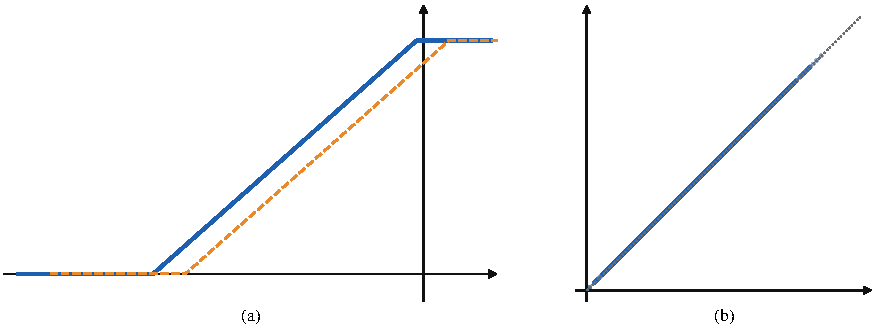
\includegraphics[width=0.9\linewidth]{figures/niezmiennik-glosnosci.pdf}
\caption{(a) Cecha jako funkcja $\log_{10}A$ (niebieska): płaski początek (cisza poniżej $60\dB$ od referencji), liniowy wzrost i przycięcie na $1{,}3$.
Nagranie 3 razy głośniejsze (pomarańczowa przerywana) ma tę samą krzywą, bo referencja przesuwa się razem z poziomami (tw.~\ref{tw:glosnosc}).
(b) Wartości cech tego samego nagrania (poziomo) i nagrania 10 razy cichszego (pion): wszystkie punkty leżą na przekątnej (kropkowana).}
\label{rys:niezmiennik}
\end{figure*}

\begin{pulapka}
Niezależność od głośności dotyczy \emph{stałego} przeskalowania całego nagrania. Nie obejmuje szumu: jeśli głośniejsza jest tylko jedna część,
albo tło ma stały poziom, normalizacja nie pomoże. Stała $10^{-9}$ w logarytmie psuje twierdzenie tylko dla amplitud tak małych, że i tak są obcięte do zera.
\end{pulapka}

\section{Kanały to przesunięte kopie jednego widma}

\begin{twierdzenie}[Przesunięcie kanałów]\label{tw:przesuniecie-kanalow}
Jeśli $k_h=36\log_2h$ jest liczbą całkowitą, to dla każdej klatki i każdego binu $p$ zachodzi $A_h[t,p]=A_1[t,p+k_h]$.
\end{twierdzenie}
\begin{pomyslDowodu}
Bin $p+k_h$ ma częstotliwość środkową dokładnie $h$ razy większą niż bin $p$, więc obie amplitudy to maksimum z tego samego przedziału widma.
\end{pomyslDowodu}
\begin{proof}
Z def.~\ref{def:bin} mamy $m_{p+k_h}=m_p+k_h/3$. Zatem
\begin{align*}
f(p+k_h) &= 440\cdot2^{(m_p+k_h/3-69)/12}=f(p)\cdot2^{k_h/36} && \pow{(dodanie wykładników)}\\
 &= f(p)\cdot2^{\log_2h}=h\,f(p). && \pow{($k_h=36\log_2h$)}
\end{align*}
Przedział w def.~\ref{def:hcqt} dla $A_h[t,p]$ to $[hf(p)2^{-1/72},\,hf(p)2^{1/72}]$, a dla $A_1[t,p+k_h]$ to $[f(p+k_h)2^{-1/72},\,f(p+k_h)2^{1/72}]$; są identyczne.
Maksimum z tego samego zbioru jest to samo. (Rozważamy tylko $p$, dla których $p+k_h$ mieści się w $0,\dots,158$.) To kończy dowód.
\end{proof}

Dla $h=0{,}5;2;4$ mamy $k_h=-36;36;72$, więc równość jest dokładna; dla $h=3$ i $5$ ($k_h=57{,}06$ i $83{,}59$) przesunięcie całkowite
jest tylko przybliżeniem, a błąd to poniżej pół bina. Sprawdziliśmy to na prawdziwym kodzie: dla kanałów $h=0{,}5;2;4$ różnica
$A_h[t,p]-A_1[t,p+k_h]$ wynosi dokładnie $0$ w całym nagraniu, a dla $h=3$ średnio $0{,}007$ (maksymalnie $0{,}18$). Ta własność uzasadnia
blok harmoniczny sieci (rozdział~\ref{rozdz:architektura}): sieć sama może „doprzesunąć” własne cechy o $k_h$ binów i uzyskać alikwoty także wyższe niż $5$.

\section{Co dokładnie dostaje sieć}

\begin{table}[ht]
\centering\small
\begin{tabular}{@{}lll@{}}
\toprule
parametr & wartość & znaczenie\\
\midrule
$f_s$ & $11\,025\Hz$ & po zmianie próbkowania\\
okna & $4096$ i $1024$ próbek & długie (wysokość), krótkie (czas)\\
krok & $256$ próbek $=23{,}2\ms$ & odstęp klatek\\
zero-padding & $\times4$ & gładsze położenie pików\\
alikwoty długie & $0{,}5;1;2;3;4;5$ & kanały $1$--$6$\\
alikwoty krótkie & $1;2;3$ & kanały $7$--$9$\\
biny & $3\times53=159$ & MIDI $36$--$88$\\
normalizacja & $99{,}5$ perc., $60\dB$, clip $1{,}3$ & def.~\ref{def:db}\\
\bottomrule
\end{tabular}
\caption{Parametry HCQT w modelu Gen~6. Wynik: $X\in\R^{T\times9\times159}$.}
\label{tab:hcqt-param}
\end{table}

\begin{figure*}[ht]
\centering
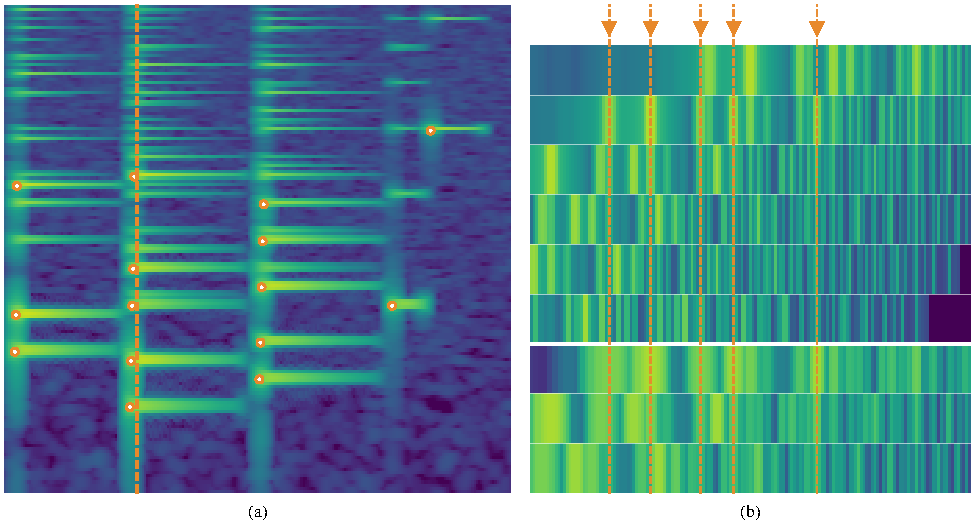
\includegraphics[width=\linewidth]{figures/hcqt-przyklad.pdf}
\caption{HCQT syntetycznego, 6-sekundowego nagrania gitary. (a) Kanał $h=1$: czas poziomo ($243$ klatki), wysokość pionowo ($159$ binów); jasne ślady to alikwoty grających nut, kółka z pomarańczowym brzegiem to początki prawdziwych nut, pomarańczowa przerywana linia to klatka pokazana w (b). (b) Cała jedna klatka: $9$ kanałów (wiersze; gruba biała linia oddziela $6$ kanałów okna długiego od $3$ okna krótkiego) $\times$ $159$ binów (kolumny). Pomarańczowe trójkąty i przerywane pionowe linie wskazują kolumny prawdziwych nut: w każdej z nich jasne plamy pojawiają się w wielu kanałach naraz, bo alikwoty kandydata ustawiono w jednej kolumnie.}
\label{rys:hcqt-przyklad}
\end{figure*}

W obu oknach analizujemy tę samą klatkę $t$ (środek wspólny). Dla nagrania 6-sekundowego $T=243$ i $X$ ma $243\cdot9\cdot159=347\,733$ liczby (przykład~\ref{prz:tensor-hcqt}).
Rysunek~\ref{rys:hcqt-przyklad}b to najważniejszy obrazek książki: siatka nut jako kolumny, siedem „pięter” alikwotów jako wiersze. Zadaniem sieci jest rozpoznać w tej siatce
wzorzec „ta kolumna jest zajęta przez nutę” i odróżnić go od kolumn, które tylko udają nutę, bo leżą oktawę niżej.

\section*{Podsumowanie}
\begin{itemize}
\item Bin wysokości ma $\tfrac13$ półtonu; $p=3s+1$ jest środkiem półtonu $s$.
\item $A_h[t,p]$ to maksimum widma wokół $hf(p)$ ($\pm\frac16$ półtonu); $h=0{,}5\dots5$ (okno długie), $1,2,3$ (krótkie): razem $9$ kanałów.
\item Cecha $=\clip((L-L_\mathrm{ref})/60+1,0,1{,}3)$ jest niezależna od głośności nagrania (tw.~\ref{tw:glosnosc}).
\item Jeśli $36\log_2h$ jest całkowite, kanał $h$ to kanał $1$ przesunięty o tyle binów (tw.~\ref{tw:przesuniecie-kanalow}).
\item Wejście sieci to $X\in\R^{T\times9\times159}$ ze krokiem $23{,}2\ms$.
\end{itemize}

\begin{sprawdz}
\begin{enumerate}
\item O ile decybeli rośnie poziom, gdy amplituda podwaja się? A gdy rośnie $10$ razy?
\item Dla $L_\mathrm{ref}=-30\dB$ policz cechę piksela o $A=0{,}005$. (Wskazówka: $L=20\log_{10}A$.)
\item Który bin odpowiada nucie A2 ($m=45$)? Jaki jest numer binu jej trzeciego alikwotu $(h=3)$, w przybliżeniu całkowitym?
\item Od jakiej wysokości kanał $h=5$ jest zerowy? Użyj progu $0{,}46f_s$ i podaj najniższy bin $p$, dla którego tak jest.
\end{enumerate}
\end{sprawdz}

\subsection*{Rozwiązania}
\begin{enumerate}
\item $20\log_{10}2=6{,}02\dB$, a $20\log_{10}10=20\dB$.
\item $L=20\log_{10}0{,}005=-46{,}02\dB$, $\varphi=(-46{,}02+30)/60+1=0{,}733$.
\item $p=3\cdot(45-36)+1=28$. Trzeci alikwot: $k_3=\round(36\log_2 3)=57$, czyli bin $28+57=85$ ($m_{85}=36+84/3=64$, to E4; dokładnie oczekiwane $45+19{,}02=64{,}02$).
\item Zero, gdy $5f(p)>5071{,}5\Hz$, czyli $f(p)>1014{,}3\Hz$, czyli $m_p>69+12\log_2(1014{,}3/440)=83{,}48$. Z $m_p=36+(p-1)/3$ dostajemy $p-1>142{,}4$, więc najniższy zerowy bin to $p=144$. Zerowych jest więc $159-144=15$ binów (najwyższe $5$ półtonów: ok.\ $83{,}5$--$88{,}3$).
\end{enumerate}
